\section{Appendix}
\subsection{File formats}
Files with extension ``ranks\_sorted''  are the actual trace results.
The fields in the table in this file:
\begin{itemize}
\item {\tt alignment\#}     number of the position in the alignment
\item {\tt residue\#}        residue number in the PDB file
\item {\tt type}            amino acid type
\item {\tt rank}            rank of the position according to older version of ET
\item {\tt variability}     has two subfields:
  \begin{enumerate}
                \item number of different amino acids appearing in
                    in this column  of the alignment
                \item  their type
  \end{enumerate}
		  
\item {\tt rho}             ET score - the smaller this value, the lesser variability
                of this position across the branches of the tree
                (and, presumably, the greater the importance for the protein)
\item {\tt cvg}             coverage - percentage of the residues on the structure which
                have this rho or smaller
\item {\tt gaps}            percentage of gaps in this column
\end{itemize}

\subsection{Color schemes used}
\begin{figure} [t]
{
  \center
  \includegraphics[width=80mm] {colorbar_horizontal.eps}
}
\caption{\label{colorbar} Coloring scheme used to color residues by their relative importance.}
\end{figure}

The following color scheme is used in figures with residues colored by  cluster size:
 black is a single-residue cluster; clusters composed of more than one residue colored according to this hierarchy 
(ordered by descending size): red, blue, yellow, green, purple, azure, turquoise, brown, coral,
               magenta, LightSalmon, SkyBlue, violet, gold, bisque, LightSlateBlue, orchid,
               RosyBrown, MediumAquamarine, DarkOliveGreen, CornflowerBlue, grey55, burlywood,
               LimeGreen, tan, DarkOrange, DeepPink, maroon, BlanchedAlmond.

The colors used to distinguish the residues by the estimated  evolutionary pressure they experience can
be seen in Fig. \ref{colorbar}.


\subsection{Credits}
%
\subsubsection{\bf Alistat}
\emph{alistat} reads a multiple sequence alignment from the file  and shows a number of simple statistics about it. 
These statistics include the format, the number of sequences, 
the total number of residues, the average and range of the sequence lengths, and the alignment length (e.g. including gap characters).
Also shown are some percent identities. A percent pairwise alignment identity is defined as (idents / MIN(len1, len2)) 
where idents is the number of exact identities and len1, len2 are the unaligned lengths of the two sequences. 
The "average percent identity", "most related pair", and "most unrelated pair" of the alignment are the average,
 maximum, and minimum of all (N)(N-1)/2 pairs, respectively. 
The "most distant seq" is calculated by finding the maximum pairwise identity 
(best relative) for all N sequences, then finding the minimum of these N numbers (hence, the most outlying sequence). 
\emph{alistat} is copyrighted by  HHMI/Washington University School of Medicine, 1992-2001,
and freely distributed under the GNU General Public License.
%
%
\subsubsection{\bf CE}
To map ligand binding sites from different source structures, report\_maker uses the CE program:
{\tt http://cl.sdsc.edu/}.
Shindyalov IN, Bourne PE (1998) \emph {"Protein structure alignment by incremental combinatorial extension (CE) of the optimal path}
. Protein Engineering 11(9) 739-747.

%
\subsubsection{\bf DSSP}
 In this work a residue is considered solvent accessible if the 
 DSSP program
  finds it exposed to water by at least 10\AA$^2$, 
which is roughly the area  needed for one water molecule
to come in the contact with the residue.
DSSP is copyrighted by 
  W. Kabsch, C. Sander and MPI-MF, 1983, 1985, 1988, 1994 1995, 
  CMBI version by Elmar.Krieger{\tt @cmbi.kun.nl} November 18,2002,
\begin{verbatim}http://www.cmbi.kun.nl/gv/dssp/descrip.html.\end{verbatim}
%
\subsubsection{\bf HSSP}
 Whenever available, report\_maker uses HSSP alignment as a starting point for the analysis
(sequences shorter than 75\% of the query are taken out, however); 
R. Schneider, A. de Daruvar, and C. Sander. 
\emph {"The HSSP database of protein structure-sequence alignments.''} Nucleic Acids Res., 25:226--230, 1997.
\begin{verbatim}http://swift.cmbi.kun.nl/swift/hssp/\end{verbatim}
%
\subsubsection{\bf LaTex}
The text for this report was processed using \LaTeX;
 Leslie Lamport, ``LaTeX: A Document Preparation System
Addison-Wesley,'' Reading, Mass. (1986).
%
\subsubsection{\bf Muscle}
When making alignments ``from scratch'', report maker uses Muscle  alignment program:
Edgar, Robert C. (2004), 
\emph {"MUSCLE: multiple sequence alignment with high accuracy and high throughput.''}
Nucleic Acids Research 32(5), 1792-97.
\begin{verbatim}http://www.drive5.com/muscle/\end{verbatim}
%
\subsubsection{\bf Pymol}
The figures in this report were produced using Pymol. The scripts can be found in the 
attachment. Pymol is an open-source application copyrighted by DeLano Scientific LLC (2005).
 For more information about Pymol see {\tt http://pymol.sourceforge.net/}.
{\small(Note for Windows users: the attached package needs to be unzipped for Pymol
to read the scripts and launch the viewer.)}

\subsection{Note about ET Viewer}
 Dan Morgan from the Lichtarge lab has developed a visualization tool specifically for
viewing trace results. If you are interested, please visit:
\begin{verbatim} http://mammoth.bcm.tmc.edu/traceview/ \end{verbatim}
The viewer is self-unpacking and self-installing.
Input files to be used with ETV (extension .etvx) can be found in the attachment to the main report.


\subsection{Citing this work}
The method used to rank residues and make predictions in this report can be found in 
Mihalek, I., I. Re\v{s}, O. Lichtarge. (2004).
\emph {"A Family of Evolution-Entropy Hybrid Methods for Ranking of Protein Residues by Importance" }
J. Mol. Bio. {\bf 336}: 1265-82.
For the original version of ET see
O. Lichtarge, H.Bourne and F. Cohen  (1996).
\emph {"An Evolutionary Trace Method Defines Binding Surfaces Common to Protein Families" }
J. Mol. Bio. {\bf 257}: 342-358.


\subsection{About report\_maker} 
{\tt \bf report\_maker} was written in 2006 by Ivana Mihalek. The 1D ranking visualization
program was written by Ivica Re\v{s}.
 {\tt \bf report\_maker} is copyrighted by Lichtarge Lab,
Baylor College of Medicine, Houston.

